\documentclass[12pt]{article}  % standard LaTeX, 12 point type

\usepackage{geometry}

\usepackage{amsmath}
\usepackage{amsfonts,latexsym}
\usepackage{amsthm}
\usepackage{amssymb}
\usepackage[utf8]{inputenc} % Кодировка
\usepackage[english,russian]{babel} % Многоязычность
\usepackage{verbatim}
\usepackage{longtable}
\usepackage{csvsimple}
\usepackage[toc,page]{appendix}
\usepackage{booktabs}

\usepackage{float}
\usepackage{array}
\usepackage{multirow}
\usepackage{caption}
\usepackage{graphicx}
\usepackage{ucs}
\usepackage{rotating}
\usepackage{pdflscape}
\usepackage{afterpage}
\usepackage{capt-of}% or use the larger `caption` package
\usepackage{url}

% unnumbered environments:

\theoremstyle{remark}
\newtheorem*{remark}{Remark}
\newtheorem*{notation}{Notation}
\newtheorem*{note}{Note}

\setlength{\parskip}{5pt plus 2pt minus 1pt}
\newcolumntype{C}{>{\centering\arraybackslash}p{1.3cm}}
\renewcommand\appendixpagename{Приложение}
\graphicspath{{pics/}}

\title{Использование КС-грамматики для распознавания \\ 16s рРНК}
\author{Семён Григорьев, Дмитрий Ковалёв}
\date{\today}

\begin{document}

\newgeometry{left=0.8in,right=0.8in,top=1in,bottom=1in}

\maketitle 

\section{Введение}

Одна из задач, возникающих в биоинформатике --- задача поиска и классификации маркерных цепочек, использующихся для обнаружения и классификации организмов.
При этом, многие маркерные цепочки обладают достаточно богатой вторичной структурой, что позволяет сделать предположение, что её можно использовать для решения данной задачи.
Более того, известно, что некоторые участки обладают достаточно консервативной вторичной структурой, например, центральный домен 16s~\cite{cons16s}.
Использование вторичной структуры при решении задач поиска и классификации цепочек не является новой идеей.
Она используется как в широко распространённых инструментах (например, Infernal~\cite{Infernal}), так и во многих теоретических исследованиях~\cite{SCFGRNA1,SCFGRNA2, STEMSEARCH1, STEMSEARCH2, SCFGHARD1}.

Вторичная структура цепочек может быть описана с помощью грамматик. 
В зависимости от требуемой точности могут использоваться разные классы грамматик: регулярные, контекстно-свободные, конъюнктивные.
В данной работе будут использоваться контекстно-свободные грамматики и соответствующий класс языков.
В результате, по аналогии с поиском по регулярному выражению, задача поиска сведётся к поиску структурного шаблона, заданного контекстно-свободной грамматикой.
Так как вторичная структура больших цепочек может быть достаточно сложной, соответствующая грамматика также оказывается сложной.
При этом часто необходимо искать баланс между сложностью грамматики, которая непосредственно связана с детализацией описания вторичной структуры, и производительностью и точностью поиска.

Одна из маркерных цепочек, часто используемая в настоящее время --- это 16s rRNA.
Данный отчёт описывает эксперимент по распознаванию 16s с использованием информации только о её вторичной структуре, описанной контекстно-свободной грамматикой.

\section{Описание вторичной структуры с помощью грамматики}

Для спецификации грамматики был использован язык YARD~\cite{YARD}, основанный на ECFG~\cite{ECFG} с различными расширениями.
В правых частях можно использовать конструкции регулярных выражений.

В таблице~\ref{tbl1} представлены основные конструкции и примитивы, использовавшиеся при написании грамматики.
Так как описание несовпадений в стеме в общем случае является сложной задачей (возможно, неразрешимой в 
терминах контекстно-свободных грамматик), были использованы такие правила, как $stem\_e1{<}s{>}$, описывающие приближение множества стемов с несовпадениями.

\begin{table}[h]
    \centering
    \renewcommand{\arraystretch}{1.5}
    \begin{tabular}{|c|>{\centering}p{9cm}|}
        \hline
        Грамматическая конструкция & Описание 
        \tabularnewline \hline
        $ any $ & Один из нуклеотидов $A, U, C, G$. 
        \tabularnewline \hline
        $ any^*[n..m] $ & Цепочка нуклеотидов длины от $n$ до $m$. 
        \tabularnewline \hline
        $stemN{<}s{>}$  & Стем высоты $N$ со свободной частью $s$ (последовательность любых конструкций грамматики). 
        \tabularnewline \hline
        $mk\_stem{<}s{>}$ & Стем произвольной высоты (от $0$ до $N$) со свободной частью $s$.
        \tabularnewline \hline
        $stem\_e1{<}s{>}$ & Стем, позволяющий одно несовпадение, при этом требующий, чтобы подряд было не менее двух парных элементов. 
        \tabularnewline \hline
    \end{tabular}    
    \caption{Базовые конструкции грамматики}
    \label{tbl1}
\end{table}

\begin{table}[h]
    \centering
    \renewcommand{\arraystretch}{2}
    \begin{tabular}{c | c}
        $stem4{<}any^*[3..5]{>}$ & $mk\_stem{<} any^*[1..2] \ stem2{<} any^*[3..4] {>} \ any^*[2..5] {>}$ \\
        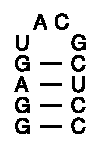
\includegraphics[width=1.5cm]{stem4.pdf} & 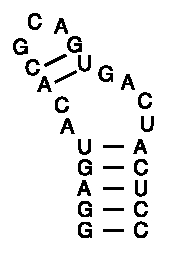
\includegraphics[width=2cm]{mk_stem.pdf} \\
    \end{tabular}
    \caption{Примеры описания структур}
\end{table}

\section{Эксперименты}

Для проведения эксперимента прежде всего необходима контекстно-свободная грамматика, описывающая вторичную структуру искомой цепочки.
Построение грамматики, задающей вторичную структуру, в настоящий момент выполняется вручную, однако возможен и вывод грамматики, но это тема для отдельного исследования.

Используемая в эксперименте грамматика, которая была построена нами, приведена в приложении \ref{grammar}.
В качестве образца была использована эталонная вторичная структура 16s Escherichia coli.
Терминальный алфавит состоит из четырех символов-нуклеотидов: $A, U, C, G$.
Для спецификации стемов активно используются параметризуемые правила, что позволяет сделать граммтику достаточно компактной.
Ключевое слово \verb|inline| является служебным и используется для того, чтобы подсказать генератору синтаксических анализаторов, как именно преобразовывать грамматику в ходе работы.

Всего было поставлено два эксперимента: обработка базы известных последовательностей 16s и поиск 16s в полноразмерных размеченных геномах.
Целью первого эксперимента была оценка качества составленной нами граммитики на предмет полноты детектирования цепочек: вычислялся процент нераспознанных цепочек относительно всех обработанных.
Цель второго --- оценка количества ложных срабатываний. Вместе с этим оценивалась и полнота поиска.

Для первого эксперимента была использована база цепочек проекта SILVA~\cite{Silva}, которая содержит более 20 тысяч различных последовательностей.
Результаты данного эксперимента приведены в таблице~\ref{16sBase}, где '+' --- количество распознанных цепочек для соответствующего домена, '-' --- количество нераспознанных.
В итоге, при использовании грамматики для центрального домена распознанно 98.16\% цепочек, являющихся 16s рРНК, а при использовании грамматики для 5'M домена --- 63.13\%. 
Кроме этого, можно заметить, что 5'M домен лучше разделяет домены.

\begin{table}[h]
    \centering
    \begin{tabular}{c >{\centering}p{3cm} *{6}{C}}
        \toprule
        \multirow{2}{*}{Домен} & \multirow{2}{*}{\parbox{3cm}{\centering Стартовый нетерминал}} & \multicolumn{2}{c}{Бактерии} & \multicolumn{2}{c}{Эукариоты} & \multicolumn{2}{c}{Археи} \\
        \cmidrule(lr){3-4}
        \cmidrule(lr){5-6}
        \cmidrule(lr){7-8}
        & & + & - & + & - & + & - \\
        \midrule
        Центральный & h19 & 17878 & 335 & 2153 & 3165 & 306 & 13 \\
        5'M & h3 & 11498 & 6715 & 64 & 5254 & 81 & 238\\
        \bottomrule
    \end{tabular}
    \caption{Результаты анализа базы организмов}
    \label{16sBase}
\end{table}

Для второго эксперимента использовались 100 размеченных геномов из базы NCBI.
Поиск по центральному домену показал очень большое количество ложных срабатываний, поэтому резуьтаты здесь приводиться не будут.
Часть результатов поиска по 5'M домену приведены в таблице~\ref{headtable}. 
В таблице указан код организма в NCBI, его название, количество размеченных и правильно обнаруженных последовательностей 16s (Expected и Covered соответственно), количество ложных срабатываний (FP-intervals), средняя длина и отклонение для цепочек, соответствующих ложным срабатваниям.
Последние два столбца могут помочь оценить объём работы по дополнительной фильтрации ложных срабатываний.
В итоге, для 100 геномов получены следующие результаты:
\begin{itemize}
\item среднее количество ложных срабатываний на геном равно 299, отклонение равно 221,54;
\item средняя доля правильно обнаруженных цепочек равна 0,98 при отклонении 0,11.
\end{itemize}

Также, в таблице~\ref{headmiddle_table} приведены результаты поиска по совмещённой грамматике для 5'M и центрального домена.
Обращает на себя резкое снижение количества ложных срабатваний.
При этом, однако, уменьшается и количество положительных совпадений.

\afterpage{
    \begin{landscape}
        \csvloop{
            file=final_report_head.csv,
            no head,              % no special treatment of first line
            column count=7,       % since no first line is given, tell about column count
            respect all,
            before reading=
                \begin{footnotesize}
                \begin{longtable}{llccccc}\footnotesize \\ \toprule,
            command=\csvlinetotablerow,
            late after line=\\,
            late after first line=\\\midrule,
            late after last line=\\\bottomrule,
            after reading=
                \caption{Результаты анализа полноразмерных геномов (5'M домен)}
                \label{headtable}
                \end{longtable}
                \end{footnotesize}
        }
        \csvloop{
            file=final_report_headmiddle.csv,
            no head,
            column count=7,
            respect all,
            before reading=
                \begin{footnotesize}
                \begin{longtable}{llccccc}\footnotesize \\ \toprule,
            command=\csvlinetotablerow,
            late after line=\\,
            late after first line=\\\midrule,
            late after last line=\\\bottomrule,
            after reading=
                \caption{Результаты анализа полноразмерных геномов (5'M + центральный домены)}
                \label{headmiddle_table}
                \end{longtable}
                \end{footnotesize}
      }
    \end{landscape}
}

\pagebreak  


\section{Заключение}

Данный эксперимент показал наличие возможности использовать вторичную структуру цепочки для предварительной фильтрации кандидатов, однако требуется существенная доработка используемых алгоритмов.
В дальнейшем планируется выполнение работ по следующим направлениям.
\begin{itemize}
\item Поиск, разработка и применение алгоритмов автоматического вывода грамматик для построения грамматики, описывающей вторичную структуру цепочки.
\item Анализ ложных срабатываний и пропущенных кандидатов с целью выявить их особенности и доработать соответствующим образом алгоритм поиска.
\item Разработка методов уменьшения количества ложных срабатываний.
\end{itemize}


\begin{thebibliography}{9}

\bibitem{Infernal}
   Nawrocki E. P., Eddy S. R. Infernal 1.1: 100-fold faster RNA homology searches //Bioinformatics. – 2013. – Т. 29. – №. 22. – С. 2933-2935.

\bibitem{SCFGRNA1}
Dowell R. D., Eddy S. R. Evaluation of several lightweight stochastic context-free grammars for RNA 
secondary structure prediction //BMC bioinformatics. --- 2004. --- Т. 5. --- \textnumero. 1. --- С. 1.

\bibitem{SCFGRNA2}
Eddy S. R. A memory-efficient dynamic programming algorithm for optimal alignment of a sequence to 
an RNA secondary structure //BMC bioinformatics. --- 2002. --- Т. 3. --- \textnumero. 1. --- С. 1.

\bibitem{STEMSEARCH1}
Yogev S., Milo N., Ziv-Ukelson M. StemSearch: RNA search tool based on stem identification and indexing //Bioinformatics and Biomedicine (BIBM), 2013 IEEE International Conference on. --- IEEE, 2013. --- С. 145-152.

\bibitem{STEMSEARCH2}
Eddy S. R. Homology searches for structural RNAs: from proof of principle to practical use //RNA. --- 2015. --- Т. 21. --- \textnumero. 4. --- С. 605-607.

\bibitem{SCFGHARD1}
Anderson J. W. J. et al. Evolving stochastic context--free grammars for RNA secondary structure prediction //BMC bioinformatics. --- 2012. --- Т. 13. --- \textnumero. 1. --- С. 78.

\bibitem{ECFG}
Hemerik K. Towards a Taxonomy for ECFG and RRPG Parsing //Language and Automata Theory and Applications. – 2009. – С. 410-421.

\bibitem{Silva}
Quast C. et al. The SILVA ribosomal RNA gene database project: improved data processing and web-based tools //Nucleic acids research. – 2012. – Т. 41. – №. D1. – С. D590-D596.

\bibitem{YARD}
YARD language description. Online. \url{http://yaccconstructor.github.io/YaccConstructor/yard.html}

\bibitem{cons16s}
Rehakova K. et al. Variation in secondary structure of the 16S rRNA molecule in cyanobacteria with implications for phylogenetic analysis //Fottea. – 2014. – Т. 14. – С. 161-178.

\end{thebibliography}

\begin{appendices}
\section{Грамматика 16S на языке YARD, использовавшаяся в эксперименте}
\label{grammar}
\verbatiminput{16S_grammar.yrd}
\end{appendices}
\end{document}